\newpage
\section{Тестирование}
\setcounter{figure}{0}

Так как для данной системы не существует спроектированных УСПД и ССД для тестирования необходимо реализовать эмуляторы УСПД и ССД. 

Программа реализована на языке C++ с использованием библиотек Qt. Qt Framework является основным инструментом для разработки ССД и СБД данной системы.

Особенностью Qt является свой подход на обработку событий. Обычно события обрабатываются в том же потоке, что и основная программа. Qt предоставляет механизм сигналов и слотов, которые обрабатываются каждый в своём потоке. Для этого в Qt реализован свой объект QApplicatin, объект которого отвечает за обработку сигналов и слотов. Так как язык C++ не предоставляет средств по работе с сигналами и слотами, в Qt есть абстрактный объект QObject, в котором реализованы макросы для правильной компиляции приложений. Данный объект содержит макросы, которые обрабатываются препроцессором и разворачивают команды работы с сигналами в конструкции, совместимые с C++.

QObject является предком для всех объектов, предоставляемых Qt, все, наследованные от него объект поддерживают использование макросов. Для создания своих объектов, со своими сигналами и слотами необходимо наследовать объекты от QObject, либо другого объекта Qt. При множественном наследовании потомком QObject может быть только один класс-предок. 

Сигналом объекта Qt является метод без реализации, который испускаетя как реакция на какой-либо определенное событие. При описании своих объектов описание сигналов происходит в специальной секцие signal. Для того, что бы испустить сигнал используется специальная команда emit.

Слот - это метод объекта, который можно вызывать как напрямую, так и после испускания определенного сигнала. Слот вызывается каждый раз, как испускается сигнал связанный с ним. Связь сигнала и слота производится при помощи команды connect. Данная команда связывает определеный сигнал определенного объекта с определенным слотом другого (или того же) объекта. Шаблон для создания своих объектов представлен ниже.

\begin{lstlisting}
 #include <QObject>
 
 class MyObject : public QObject
 {
   Q_OBJECT
 public:
   explicit MyObject(QObject *parent = 0);
   ~MyObject();
   
 signals:
   void newVal();
   
 slots:
   void setVal(int val);
   
 private:
   int value;
 };
\end{lstlisting}

Сетевое взаимодействие в программах, написанных на языке C++ реализуется при помощи сокетов\cite{cpp}, в Qt для реализации данного взаимодействия используется надстройка над механизмом сокетов, облегчающая реализацию данного взаимодействия.

Данный механизм представлен такими классами как \cite{qt}:
\begin{itemize}
 \item QAbstrackSocket;
 \item QTcpSocket;
 \item QTcpServer;
 \item QUdpSocket.
\end{itemize}

QTcpServer - это объект, предназначенный для обработки сетевых подключений к определенному порту сетевого интерфейса. Задачами объектов типа QTcpServer является прослушивание указанного порта. При появлении входящего подключения данный объект реагирует на это событие созданием объекта QTcpSocket, который отвечает за отправку данных клиенту. 

При появлении подключения объектов типа QTcpServer испускает сигнал newConnection. Данный сигнал связывается с обработчиком новых подключений, в котором создается объект типа QTcpSocket в конструктор которого подается ссылка на сокет, полученная при помощи метода nextPendingConnection() объекта типа QTcpServer. 

Пример обработки нового подключения представлен в листинге ниже.

\begin{lstlisting}
 MyServer::MyServer(const *int port)
 {
   srv->listen(QHostAddress::Any, port);
   connect(srv, SIGNAL(newConnection()), this, SLOT(newConnect()));
 }
 
 void MyServer::newConnect()
 {
   sc = new QTcpSocket(srv->nextPendingConnection());
   connect(sc, SIGNAL(readyRead()), this, SLOT(readData()));
 }
 
 void MyServer::readData()
 {
   QByteArray buf(sc->readAll());
   qDebug() << QString(buf);
 }
\end{lstlisting}

В данном примере осуществляется инициализация объекта типа QTcpServer и связывание события появления нового подключения с его обработчиком newConnect(). В обработчике инициализируется объект типа QTcpSocket и происходит связь события о получении данных с его обработчиком readData(). В обработчике readData() происходит считывание всех данных из сокета и выводит их в консоль.

QTcpSocket - это объект, предназначенный для отправления данных при помощи протокола TCP. Объекты данного типа связываются с определенным портом определенного хоста и отправляют данные на этот порт ожидая. Объекты данного типа имеют методы для отправки данных клиенту и сигналы об окончании передачи данных, о наличии новых принятых данных, о разрыве соединения и др.

Для работы с объектом типа QTcpSocket необходимо реализовать обработчики событий. В примере ниже приведен пример использования объектов типа QTcpSocket для создания соединения с удаленным хостом, отправки данных и получения ответа от хоста.

\begin{lstlisting}
 MySocket::MySocket(const *QString addr, const *int, port)
 {
   sc = new QTcpSocket(this);
   sc->connectToHost(addr, port);
   connect(sc, SIGNAL(readyRead()), this, SLOT(getData()));
 }
 
 void MySocket::sendData(QByteArray data)
 {
   sc->write(data);
 }
 
 void MySocket::getData()
 {
   QByteArray buf(sc->readAll());
   qDebug() << QString(buf);
 }
\end{lstlisting}

В данном примере создается сокет, который подключается к указанному хосту, а так же связывает сигнал readyRead() со слотом getData(). Слот getData() предназначен для получения данных от хоста и вывода их в консоль. Метод sendData(QByteArray data) отправляет массив данных хосту.

\subsection{Эмулятор УСПД}

Для основы эмулятора УСПД был выбран одноплатный компьютер Raspberry Pi B+ под управлением операционной системы Raspbian. Для данного устройство разработана программа, которая ожидает подключения и при появлении запроса на отправку данных формирует пакет со сгенерированными данными в формате, описанном в разделе ``выходные данные'' данной пояснительной записки.

Для реализации взаимодействия будут использоваться классы QTcpSocket и QTcpServer.

Так как УСПД является ведомым, оно должно ожидать подключения, для открытия порта, ожидающего подключения необходимо использовать объект QTcpServer. Прототип объекта, решающего это задачу, представлен ниже.

\begin{lstlisting}
 class TestServ : public QObject
{
    Q_OBJECT
public:
    explicit TestServ(QObject *parent = 0);
    ~TestServ();
    void initServ(const int &port);

private:
    QTcpServer *srv;

public slots:
    void newConnection();
};
\end{lstlisting}

Метод initServ предназначен для запуска сервера на определенному порту, передаваемом как аргумент метода.

\begin{lstlisting}
void TestServ::initServ(const int &port)
{
    if(srv->listen(QHostAddress::Any, port))
    {
        std::cout << "server up!" << std::endl;
    }
    else
    {
        std::cout << "ooooooooooops!!!!!" << std::endl;
    }
}
\end{lstlisting}

Слот newConnection срабатывает при подключении к серверу и создает новый объект типа ClienSock для обмена данными с подключенным пользователем.

\begin{lstlisting}
void TestServ::newConnection()
{
    std::cout << "get connection =)" << std::endl;
    ClientSock * sock = new ClientSock(srv->nextPendingConnection());
    connect(sock, SIGNAL(scDisconnect(QString)), this, SLOT(connectClosed(QString)));
    users.insert(sock->getName(), sock);
}
\end{lstlisting}

Прототип объекта ClienSock:

\begin{lstlisting}
 class ClientSock : public QObject
{
    Q_OBJECT
public:
    explicit ClientSock(QTcpSocket *sock, QObject *parent = 0);
    ~ClientSock();
    void sendData(QByteArray data);
    
private:
    QTcpSocket * sc;

public slots:
    QByteArray getData();
};
\end{lstlisting}

В конструкторе создается копия сокета, по которому происходит обмен данными с клиентом.

\begin{lstlisting}
ClientSock::ClientSock(QTcpSocket *sock, QObject *parent) :
    QObject(parent)
{
    sc = sock;
    this->setName(QString("%1").arg(sock->peerPort()));
    connect(sc, SIGNAL(readyRead()), this, SLOT(getData()));
    startTimer(5000);
}
\end{lstlisting}

Слот getData срабатывает при получении данных от клиента. После чего запрос обрабатывается и происходит отправка ответа.

\begin{lstlisting}
QByteArray ClientSock::getData()
{
    QByteArray buf(sc->readAll());
    std::cout << m_qsScName.toStdString() << ": " << QString(buf).toStdString() << std::endl;
    quint16 uspdId = 0x0003;
    QString uspdData("it's USPD status");
    QString uuData("it's UU data");
    QByteArray responce;
    QDataStream res(&responce, QIODevice::WriteOnly);
    res << uspdId << uspdData.toUtf8() << uuData.toUtf8();
    sendData(responce);
    this->deleteLater();
    return buf;
}
\end{lstlisting}

Метод sendData отправляет массив байт клиенту.

\begin{lstlisting}
void ClientSock::sendData(QByteArray data)
{
    if(sc->state() == QAbstractSocket::ConnectedState)
    {
        sc->write(data);
        sc->waitForBytesWritten();
    }
} 
\end{lstlisting}

Так как данная программа только эмулирует действия УСПД, присвоим ему ID = 3, состояние УСПД представим строкой символов ``it's USPD status'', а показания УУ строкой символов ``it's UU data''.

\subsection{Эмулятор ССД}

На сервере хранится список пользователей, которых поочередно опрашивает сервер. Данный список необходимо читать и редактировать.

Для решения данной задачи необходимо создать класс, описывающий объект-сервер, который будет хранить список клиентов и выполнять опрос клиентов.

На данный момент нет описания к системе команд УСПД, поэтому ограничимся передачей любого тестового сообщения клиенту при помощи реализованных ранее классов-сокетов.

Прототип класса-сервера представлен ниже:

\begin{lstlisting}
class MyServer : public QObject
{
    Q_OBJECT
public:
    explicit MyServer(QObject *parent = 0);
    ~MyServer();

    void addClient(const QString &name, 
		   const QString &addr, 
		   const int &port);
    QMap<QString, ClientAddress>* getClientsList();

private:
    QMap<QString, ClientAddress> clients;
    void timerEvent(QTimerEvent* event);
};
\end{lstlisting}

В конструкторе данного класса запускается таймер, которй отсчитывает интервалы времени между опросами списка клиентов. 

\begin{lstlisting}
MyServer::MyServer(QObject *parent) :
    QObject(parent)
{
    startTimer(10000);
}
\end{lstlisting}

При обнулении таймера вызывается метод timerEvent в котором и происходит опрос списка клиентов, хранящегося в QMap<QString, ClientAddress>, ClientAddress - структура данных, хранящая ip-адрес и порт назначения.

timerEvent - метод, который просматривает список клиентов, для каждого клиента создает свое объект типа ClienSock(описан ранее), посылает клиенту массив байт, и отключается. 

\begin{lstlisting}
void MyServer::timerEvent(QTimerEvent *event)
{
    std::cout << "event!" << std::endl;
    foreach (QString name, this->clients.keys())
    {
        ClientSock* sc = new ClientSock(clients.value(name).addr, clients.value(name).port);
        sc->setName(name);
        sc->sendData("get_request");
    }
}
\end{lstlisting}

Метод addClient принимает имея, ip-адрес и порт клиента, которого необходимо добавить в список и создает новый элемент в объекте clients.

\begin{lstlisting}
 void MyServer::addClient(const QString &name,
                         const QString &addr,
                         const int &port)
{
    clients.insert(name, ClientAddress(addr, port));
}
\end{lstlisting}

getClientsList - метод, возвращающий атрибут clients.

\begin{lstlisting}
QMap<QString, ClientAddress>* MyServer::getClientsList()
{
    return &clients;
}
\end{lstlisting}

Графический интерфейс программы представлен на рисунку \ref{server_gui:server_gui}.

\begin{figure}[ht!]
 \center{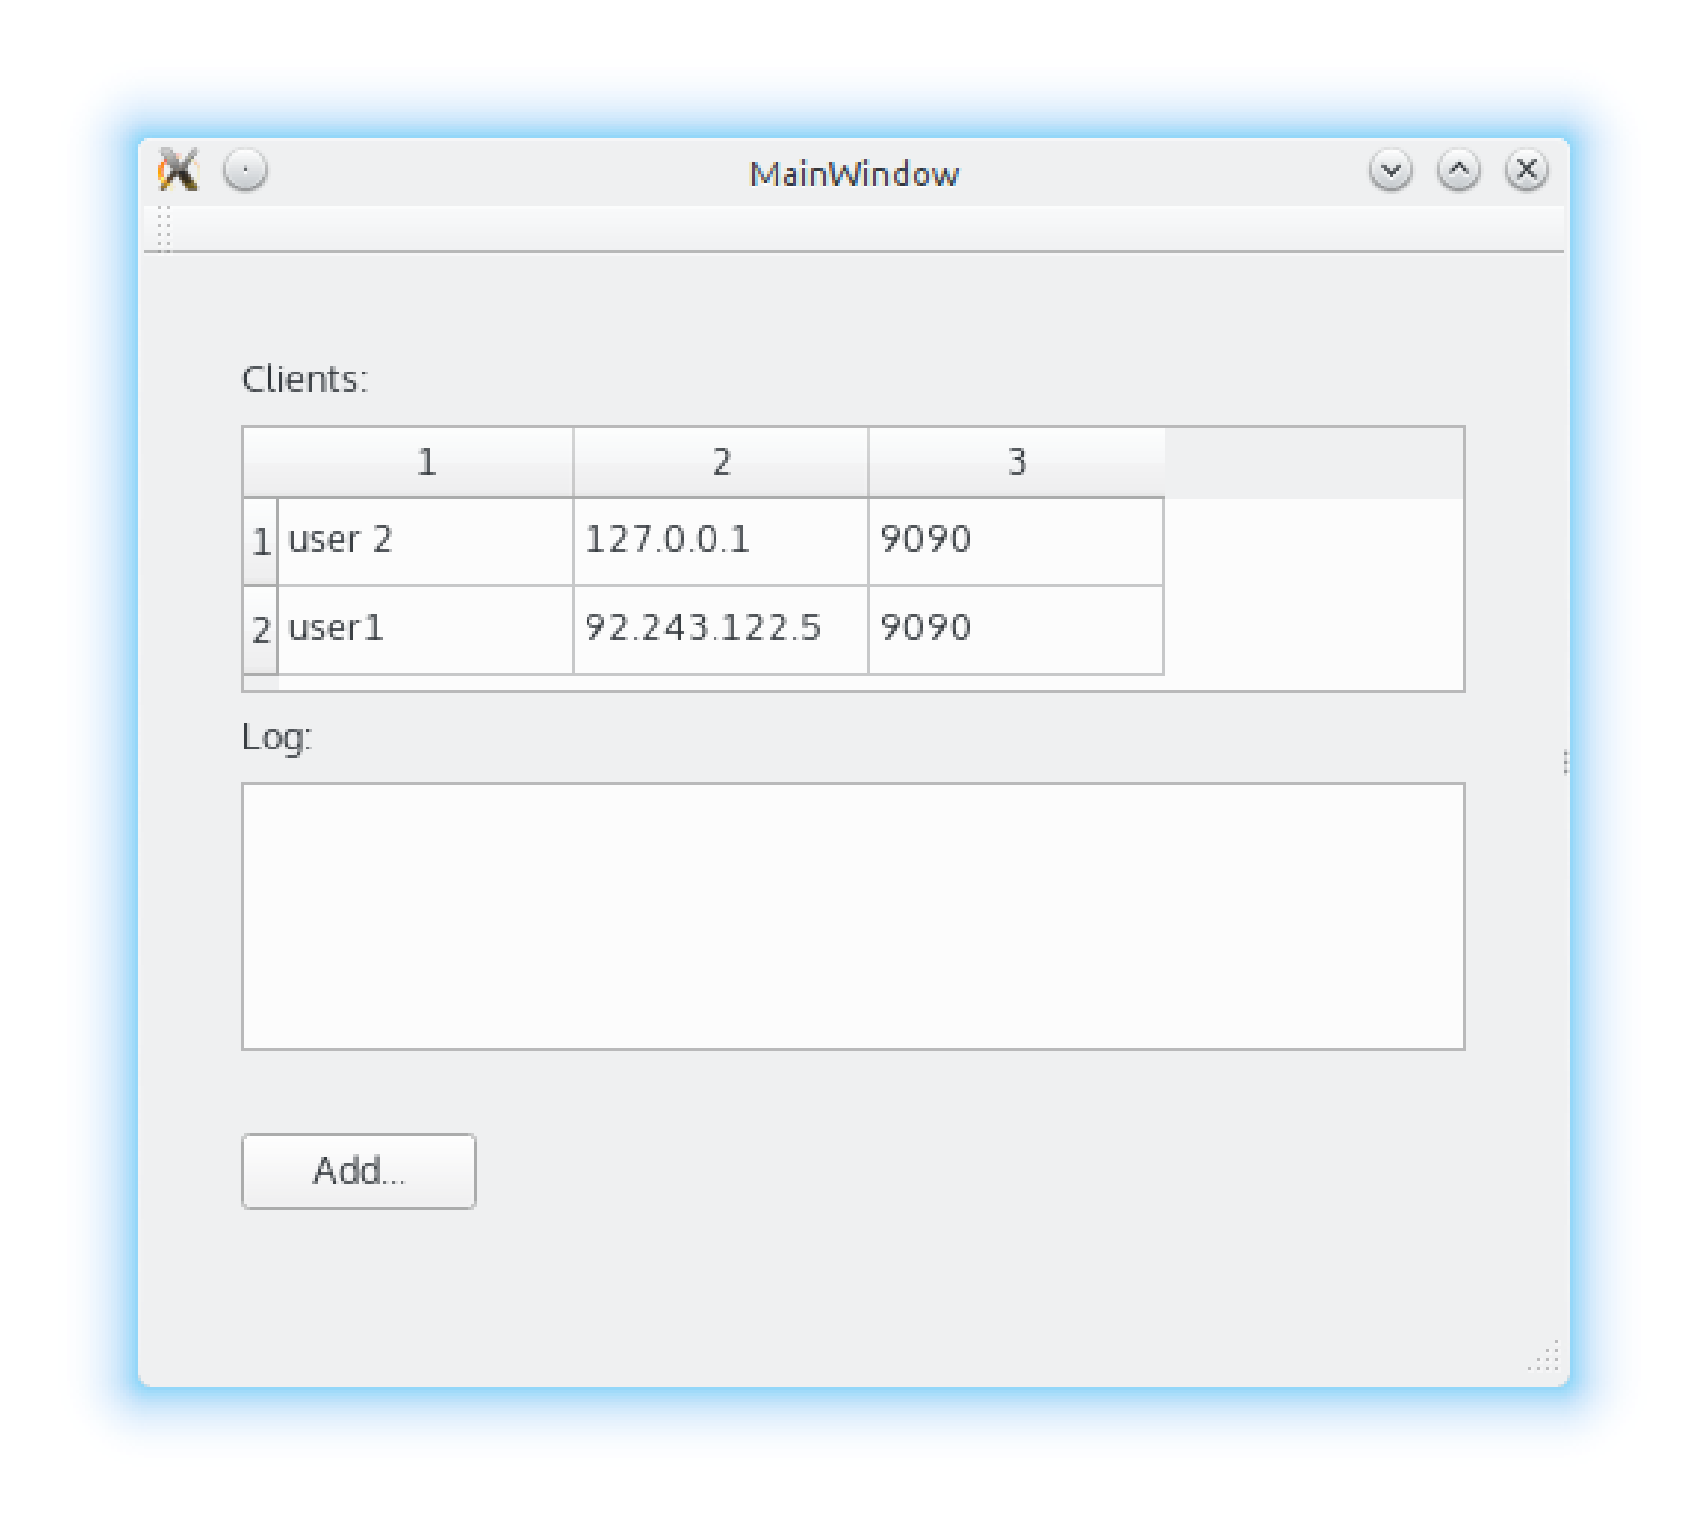
\includegraphics[width=0.7\linewidth]{server_gui}}
 \caption{Интерфейс программы}
 \label{server_gui:server_gui}
\end{figure}

\newpage
Реакция эмулятора УСПД на user1 представлена на рисунке \ref{client_log:client_log}.

\begin{figure}[ht!]
 \center{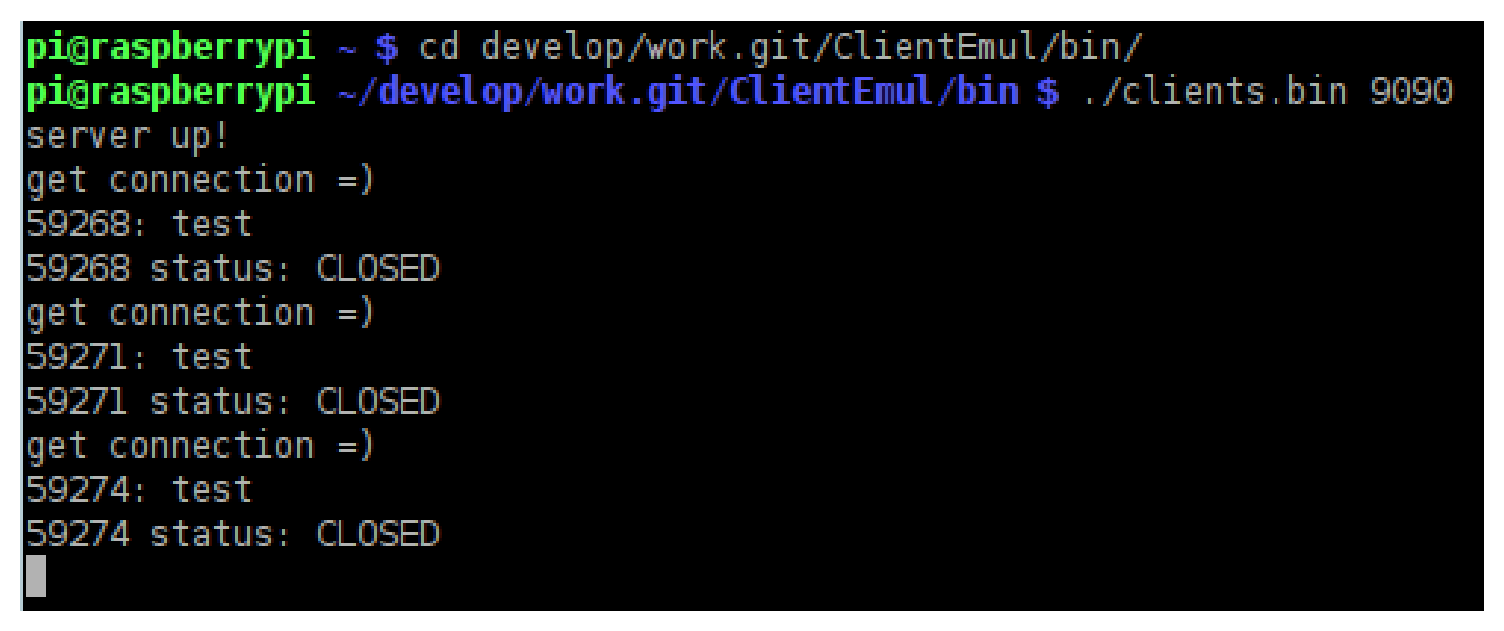
\includegraphics[width=0.7\linewidth]{client_log}}
 \caption{Работа эмулятора УСПД}
 \label{client_log:client_log}
\end{figure}

\subsection{Проверка формирования пакетов}

Для тестирования работы протокола запустим эмулятор УСПД, после чего запустим эмулятор ССД и введем адрес УСПД. Запустим wireshark\cite{nix} и дождемся очередного цикла опроса. После чего восстановим TCP сессию и рассмотрим структуру ответа. Структура ответа представлена на рисунке \ref{img:test_pachete}.

\begin{figure}[ht!]
 \center{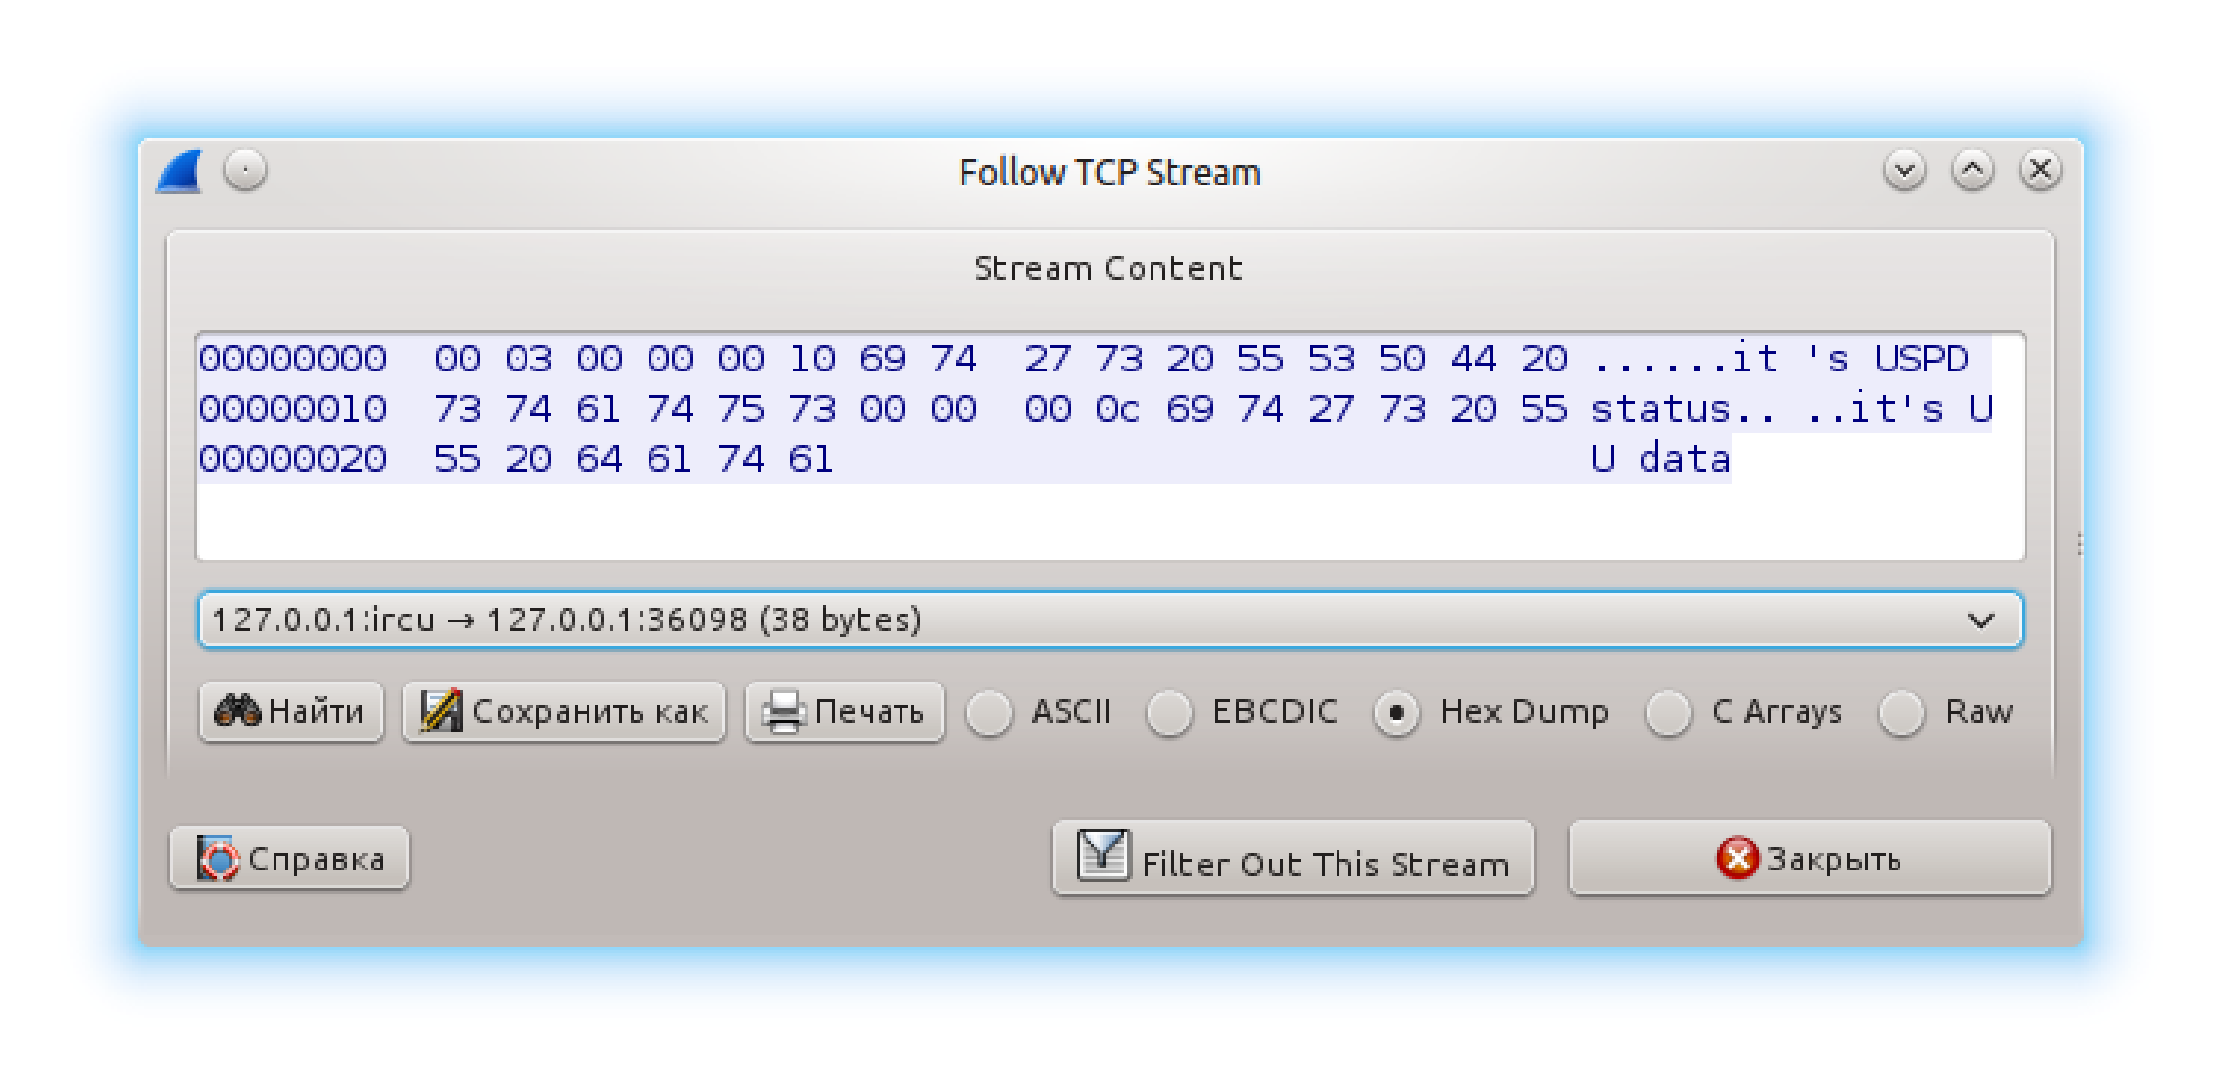
\includegraphics[width=0.7\linewidth]{test_pachete}}
 \caption{Ответ УСПД}
 \label{img:test_pachete}
\end{figure}

На рисунке представлена часть с ответом УСПД восстановленной TCP-сессии между эмуляторами. Разберем структура по байтам:

\begin{itemize}
 \item 00 03 - первые два байта, двухбайтовый ID УСПД. Совпадает с тестовыми данными УСПД;
 \item 00 00 00 10 - 4 байта - размер блока информации о состоянии УСПД. Равен 16;
 \item На рисунке видно что следующие 16 байт составляют строку состояния УСПД указанную в эмуляторе;
 \item 00 00 00 0с - 4 байта - размер блока информации от устройств учетаю Равен 12;
 \item На рисунке видно что следующие 12 байт составляют строку данных УУ указанную в эмуляторе.
\end{itemize}

На основании разбора можно сделать вывод что сформированный пакет совпадает со структурой пакета, описанной в разделе ``выходные данные''.

